%%%%%%%%%%%%%%%%%%%%%%%%%%%%%%%%%%%%%%%%%%%%%%%%%%%%%%%%%%%%%%%%%%%%%%%%
%                                                                      %
%     File: Thesis_Introduction.tex                                    %
%     Tex Master: Thesis.tex                                           %
%                                                                      %
%     Author: Andre C. Marta                                           %
%     Last modified : 13 May 2019                                      %
%                                                                      %
%%%%%%%%%%%%%%%%%%%%%%%%%%%%%%%%%%%%%%%%%%%%%%%%%%%%%%%%%%%%%%%%%%%%%%%%

\chapter{Introduction}
\label{chapter:introduction}

%%%%%%%%%%%%%%%%%%%%%%%%%%%%%%%%%%%%%%%%%%%%%%%%%%%%%%%%%%%%%%%%%%%%%%%%
\section{Motivation}
\label{section:motivation}

General relativity, developed by Albert Einstein, is a comprehensive theory of gravitation that fundamentally alters our understanding of the force of gravity. It portrays gravity not as a traditional force, but rather as a consequence of the curvature of spacetime caused by the presence of mass and energy. According to this theory, objects move through spacetime along paths dictated by this curvature, giving rise to the illusion of gravitational force.
\\
One intriguing prediction of general relativity is the existence of black holes, celestial objects with such immense gravitational pull that nothing, not even light, can escape their grasp. In the context of general relativity, the presence of a black hole causes spacetime to contort and deform, leading to bizarre phenomena like time dilation and the bending of light rays. To an observer located at a significant distance from a black hole, its appearance is analogous to that of a classical particle. This resemblance allows us to characterize a black hole by three primary quantities: its total mass, electrical charge, and spin. Remarkably, black holes that possess identical properties are indistinguishable, as no measurements can be made to discern their uniqueness \cite{HawMalStr16} — a concept known as the "No Hair" theorem.
\\
Understanding how different objects interact with black holes requires an exploration of the conservation laws that govern their behavior. By observing the initial and final state of an object that falls into a black hole, we can deduce a few of its properties through the lens of conservation. However, the reductionist nature of black holes poses a challenge—the wealth of information carried by stars and planets of various shapes and sizes is reduced to a mere three numbers. Consequently, a significant amount of information is lost, leading to a perplexing conundrum known as the information paradox \cite{HawMalStr16}.
\\
Expanding upon the topic, it is crucial to consider binary systems as significant sources of gravitational waves. Gravitational waves are ripples in the fabric of spacetime that propagate outward, carrying energy away from their source. Binary systems, composed of two massive objects orbiting around each other, emit gravitational waves as a result of their orbital motion. These waves can be detected and studied, providing valuable insights into the dynamics of spacetime and further confirming the predictions of general relativity.
\\
In the study of dynamical spacetime, researchers investigate the behavior of spacetime itself when subjected to the presence of matter and energy. The dynamics of spacetime can be studied by employing mathematical frameworks such as the theory of general relativity. By understanding the intricate interplay between matter, energy, and spacetime curvature, scientists gain a deeper understanding of how the fabric of the universe evolves and changes in response to different physical phenomena \cite{DaiVal02}.
\\
In summary, general relativity revolutionizes our comprehension of gravity by describing it as a consequence of spacetime curvature caused by mass and energy. Black holes, characterized by their immense gravitational pull, serve as fascinating objects that challenge our understanding of information conservation. The information paradox arises from the reduction of complex objects to a mere three numbers, leading to the potential loss of vast amounts of information. However, recent theories like soft "hair" propose avenues for exploring the consumption history of black holes and potentially resolving the information paradox. Additionally, binary systems play a crucial role in generating gravitational waves, allowing us to probe the dynamics of spacetime and deepen our understanding of the universe's fundamental nature. For general relativity, the definition of infinity is complicated as it has to surpass the ambiguity when discussing coordinate dependent notions and because there exist different types of infinities. In these report we will focus on only two types: null-infinity denoted by $\mathscr{I}$ and spatial infinity denoted by the symbol $i^0$.


%%%%%%%%%%%%%%%%%%%%%%%%%%%%%%%%%%%%%%%%%%%%%%%%%%%%%%%%%%%%%%%%%%%%%%%%
\section{Global structure of spacetimes}
\label{section:overview}

Roger Penrose brought to the field of general relativity the notion of conformal transformation, which made a significant impact in the geometric understanding of infinity. This was crucial for the development of theory of asymptotics, which arises a question of whether a smooth conformal extension which attaches a boundary - conformal boundary represents points at infinity - to the spacetime is shared by a larger class of spacetimes. This question leads to the notion of \textit{asymptotic simplicity} \cite{Val16}. In the context of asymptotic simplicity, spatial infinity (denoted as $i^0$) represents the region at an infinite distance from the central object or system under consideration. It provides a framework to analyze the properties of spacetime far away from the gravitational source. Similarly, null infinity (denoted as $\mathscr{I}$) represents the region at an infinite "time" in the future or past. It corresponds to the points reached by light rays that have traveled an infinite distance from their source. This simplicity allows for the application of mathematical techniques and tools to study the behavior of physical fields, gravitational waves, and the conservation laws in these simplified regimes.
Asymptotic simplicity is a concept in general relativity that refers to the behavior of spacetime at infinity. It characterizes the way spacetime and its geometry approach a simple and well-defined structure as we move to spatial infinity or null infinity.
\\
The geometric understanding of infinity also contributed to the development of gravitational radiation, taking a step forward in the mathematical understanding of gravitational waves. Although, customary in numerical approaches to general relativity, wave forms are computed at large radius, from first principles point of view they should be computed at null infinity $\mathscr{I}$. To do so, the Einstein field equations need to be expressed in terms of suitably rescaled fields, so one can evaluate the fields at $\mathscr{I}$. Technically this is done by a conformal transformation. In general relativity, conformal transformations are used to describe the behavior of physical systems under changes in the scale of spacetime. These transformations preserve the local structure of spacetime, but not necessarily its overall shape. The original metric, which we refer to as the physical metric, is denoted by $\tilde{g}$. We consider a transformation to an unphysical metric, $g$, which is given by 
\begin{equation}\label{eq:conftrans}
	g_{ab} = \Xi^2 \tilde{g}_{ab},
\end{equation}
$\Xi$ is a smooth function that approaches zero as the distance from the source increases. This transformation, denoted by \eqref{eq:conftrans}, preserves angles, making it appropriate to describe it as conformal. H. Friedrich introduced the \textit{conformal Einstein field
equations} (CEFE), a formulation designed that is in accordance with
the approach of R. Penrose.
\medskip

A prototypical example is the conformal extension of the Minkowski spacetime which will be discussed in the following.  One starts with the Minkowski metric line-element,
\begin{equation}\label{eq:metricMink-tr}
	d \tilde{s}^2=-d \tilde{t}^2+d \tilde{r}^2+\tilde{r}^2 d
        \Omega^2,
\end{equation}
where $(\tilde{t}, \tilde{r})$ $\in$ $(-\infty,+\infty) \times[0,+\infty)$ and $d \Omega^2$ represents the standard metric on $\mathbb{S}^2$. To get a conformal extension we need to do a coordinate transformation, corresponding to the advance and retarded  times, $\tilde{u}=\tilde{t}-\tilde{r}$ $\&$ $\tilde{v}=\tilde{t}+\tilde{r}$,  substituting equation \eqref{eq:metricMink-tr}.
\begin{equation}\label{eq:metricMink-tr1}
	d \tilde{s}^2=-d \tilde{u} d \tilde{v}+\frac{(\tilde{u}-\tilde{v})^2}{4} d \Omega^2.
\end{equation}
For the compactification, we need to introduce the following: $u = \tan U$ $\&$ $v = \tan V$, where $U$, $V$ $\in$ $(- \pi/2, \pi/2)$. Now, we are able to identify the conformal metric,
$ds$. Using \eqref{eq:metricMink-tr}, we obtain
$$d s^2=-4 d U d V+\sin ^2(V-U) d \Omega^2$$ where
$$d s^2=\Xi^2 d \tilde{s}^2$$
with $\Xi=2 \cos U \cos V$. Given the
domain of $U$ and $V$, we introduce the following, $T=V+U$ $\&$ $\psi=V-U$. The domain of $(T, \psi)$ is $(-\pi, \pi)$, with
\begin{equation}\label{eq:metricMink-cf}
	d s^2=-d T^2+d \psi^2+\sin ^2 \psi d \Omega^2,
\end{equation}
which is the metric of the Einstein static universe. The conformal boundary is given by $\psi = \pi/2$, which is the cylinder $\mathbb{S}^1 \times \mathbb{S}^2$, the Einstein Cylinder. The purpose of this thesis is  to study what happens at infinity, and in order to do that we will focus on the region where $\Xi = 0$. This condition gives us the following regions, which are presented in the following table
\begin{center}
    \begin{tabular}{ |c|c|c| }
      \hline
      Region & Name & Symbol \\
     \hline
     $\tilde{r} \rightarrow \infty \enspace \;  \text{with} \; \;\;\;\;
     |\tilde{t}| $<$ \infty$ & Spatial Infinity & $i^{0}$ \\
     \hline 
     $\tilde{t} \rightarrow \pm \infty$  \;\; with \;\; $\tilde{r}$<$\infty$
     \enspace & Future/Past Timelike Infinity & $i^{\pm}$ \\
     \hline
     $\tilde{r} \rightarrow \infty, \enspace \tilde{t} \rightarrow \infty \enspace
     \text{with} \;\; |u|$<$\infty$ &  Future Null-infinity & $\mathscr{I}^+$ \\ 
     \hline
     $\tilde{r} \rightarrow\infty, \enspace \tilde{t} \rightarrow-\infty \;\;
     \text{with} \enspace |v|$<$\infty$ & Past Null-infinity & $\mathscr{I}^-$ \\
     \hline
    \end{tabular}
    \end{center}
The visual representation of this is a Penrose Diagram, depicted in Fig.1
\begin{figure}[h]
	\centering 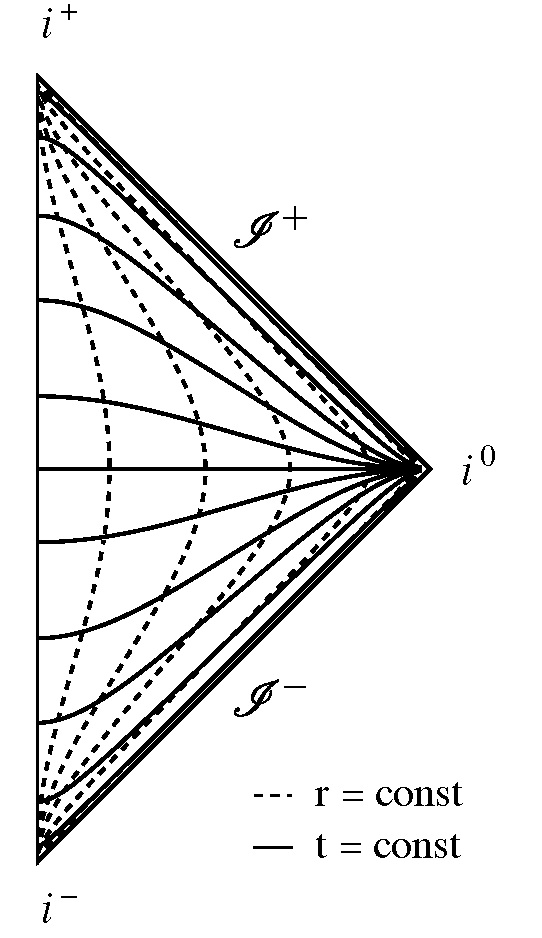
\includegraphics[width =0.3\textwidth]{Penrose diagram.pdf}
    \caption{Penrose Diagram - Representation of the standard
      compactification of the Minkowski spacetime alongside the curves of constant
      time, solid black lines, and the curves of constant r, dotted
      black lines.}
\end{figure}




%%%%%%%%%%%%%%%%%%%%%%%%%%%%%%%%%%%%%%%%%%%%%%%%%%%%%%%%%%%%%%%%%%%%%%%%
\section{Newman-Penrose Constants}
\label{section:objectives}


%%%%%%%%%%%%%%%%%%%%%%%%%%%%%%%%%%%%%%%%%%%%%%%%%%%%%%%%%%%%%%%%%%%%%%%%




